Instead of using invariant mass of four leptons $m_{4l}$, histogram templates that were generated via simulation directly in the measurements, analytical shapes are considered that have the precedence of smoothing out the irregularities because of finite number of simulated events. For measuring $m_H$, or any other physics parameter for specific $m_H$ value, signal predictions as a function of $m_H$ are continuously parameterized first, based on the simulated MC samples values of that particular $m_H$ value.
\section{Signal Modelling Methodology}
\label{section:smm}
In order to take measurements in the on-shell region production of Higgs H(125), this analysis exploits the $105 < m_{4l} < 140$ GeV range, and is then parameterized in the range $118 < m_H <130$ GeV using five mass points of $m_H$ : 120, 124, 125, 126 and 130 GeV.
The probability density function (PDF) used to model the signal shapes
for different masses in every event category were explained earlier in section \ref{section:ec}.\\
To explain the signal PDF for $m_{4l}$ with an appropriate corresponding analytical function, one must consider both the experimental results and theoretical predictions. For small $m_H$ values, a narrow-width resonance hypothesis (that a relativistic Breit-Wigner function defines the theoretical signal line shape) holds. Also taken into account are the ECAL energy leakages, experimental resolution effects such as bremsstrahlung tails in the distributions and final state radiations.
The main reason for allocation of double-sided Crystal Ball (dCB) is that it takes in consideration; both the Gaussian resolution for the core region in $m_{4l}$ distribution, and also left right asymmetric end tails given by the power-law.
\subsection{Signal Line Shape}
A Double Crystal-Ball function $f_{dCB} (m_{4l} | m_H )$ as defined in \ref{section:dcb} is the fitting strategy used to deal with this situation, we have used the linear approximation of all the Double Crystal Ball parameters varying with $m_H$. All the six parameters ``$params$'' depend on $m_H$ and are calculated for each final state and event category.
\begin{equation}
    params = params_{CB0} + params_{CB1} \times (m_H - 125 GeV)
\end{equation}
In each final state, first $params_{CB0}$ parameters are gathered from the shapes using untagged category of $ggH$ production mode at $m_H$ = 125 GeV. The shape for every end state from this are shown in Fig.\ref{fig:smm}, which also illustrates that the resolution of muons is better than electrons. Subsequently, the $params_{CB1}$ parameters are calculated, a simultaneous fit is drawn for all other $m_H$ values. One should note, that we see no significant contrast between $ggH$ and $VBF$ signal shapes in rest of the categories. This is because they have very similar branching ratios when normalised but the parametrization done from production mode of $ggH$ for untagged event category is chosen for statistically limited cases.
\begin{figure}
    \centering
    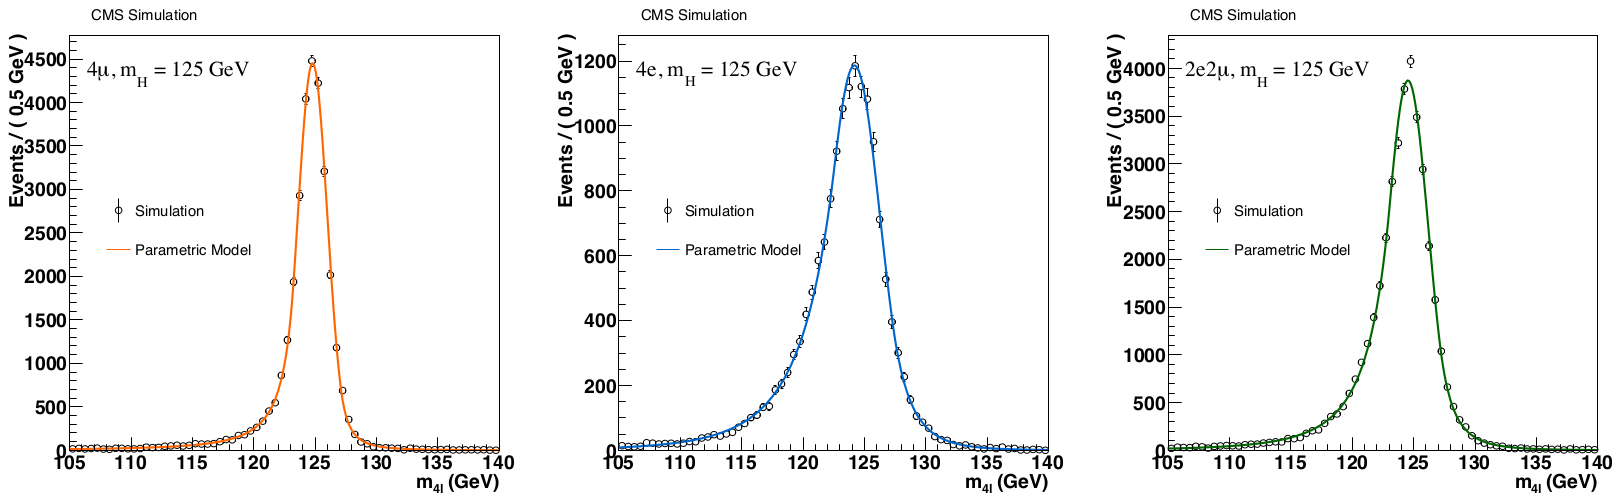
\includegraphics[scale=0.285]{images/sm.png}
    \caption{Probability density functions $f(m_{4l} |m_H)$ for ggH signal with $m_H$ =125 GeV after the full lepton and event selection. MC samples are fitted with the distributions defined in the text for $4\mu$ (left), 4e (center) and 2e2$\mu$ (right) events.}
    \label{fig:smm}
\end{figure}
In this way a unique PDF, extracted from the $ggH$ MC distribution, is valid for all the production mechanisms and categories. To check the quality of the
fits the Pull distributions as described in section \ref{section:pd} and ratio plots from Cauchy distribution described in section \ref{section:bwd} are also shown in Fig.\ref{fig:smm2}, showing an approximate Gaussian trend. The statement that pull distributions are expected to be standard Gaussian explained in section \ref{section:gd} implies a properly constructed parameterization for the simulated samples.\\
\begin{figure}[h]
    \centering
    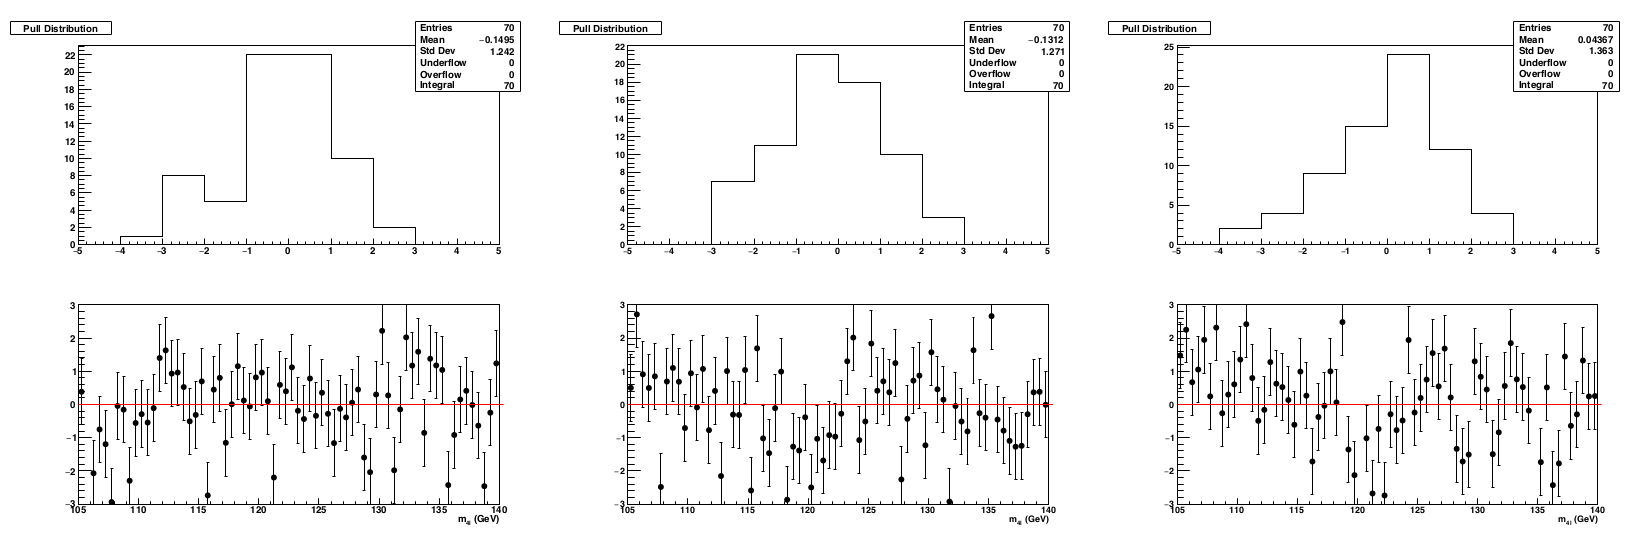
\includegraphics[scale=0.25]{images/sm2.png}
    \caption{Pull distribution (top) and the ratio distribution (bottom) for ggH signal with $m_H$ =130 GeV for 4$\mu$ (left), 4e (center) and 2e2$\mu$ (right) events.}
    \label{fig:smm2}
\end{figure}
For processes such as $WH, ZH,$ and $t\Paqt H$, the dislocated four leptons add a non-resonant component from interactions to the Higgs boson peak. A Landau function defined in section \ref{section:ld} is therefore included in the $dCB$ to perform the fit in the $m_H$ = 125 GeV case, which causes addition of two parameters, location parameter (which tells you where on the horizontal axis a graph is centered, relative to the standard normal model) and scale parameter (stretches or squeezes the graph), adjusted for simultaneous fitting. A normalization relative to each of both parameters is fixed for every category. Models fitted for all processes in each category using data of 2016, 2017 and 2018 are shown in Figure.\ref{fig:2016}, \ref{fig:2017} and \ref{fig:2018}.
\begin{figure}
    \centering
    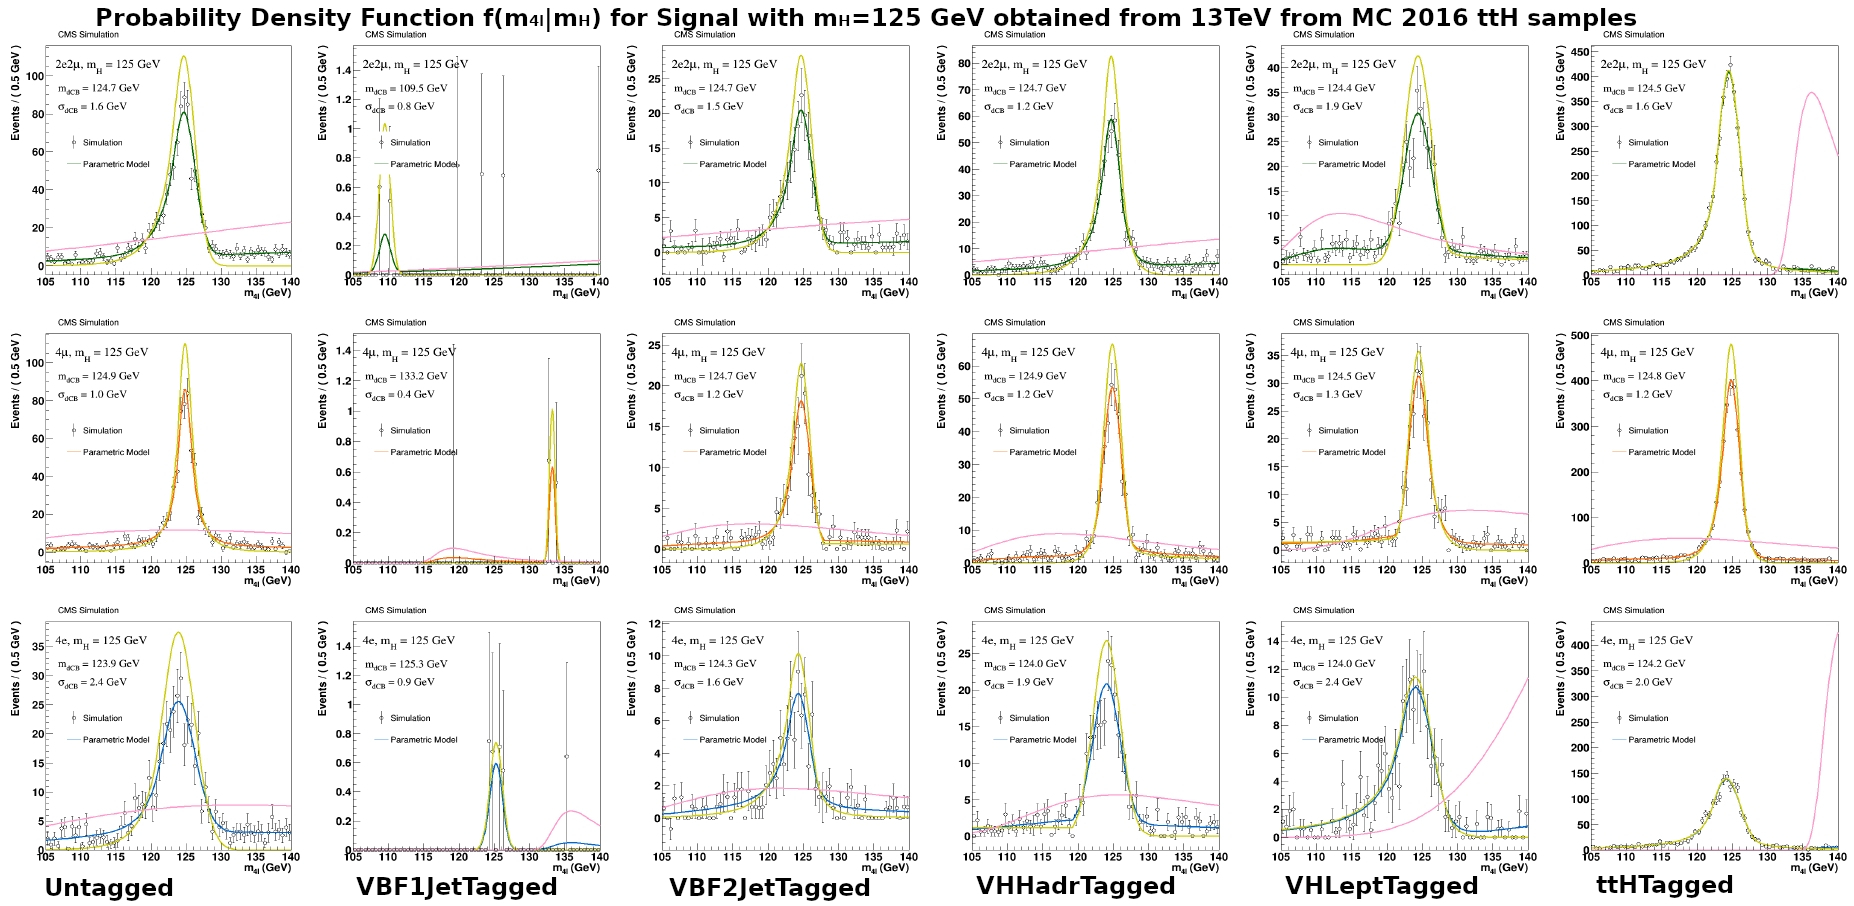
\includegraphics[scale=1]{images/2016.jpg} 
    \caption{Sum of probability density functions $f(m_{4l} |m_H)$ for $m_H$ =125 GeV fitted for 13TeV ttH 2016 MC samples.}
    \label{fig:2016}
\end{figure}
\begin{figure}
    \centering
    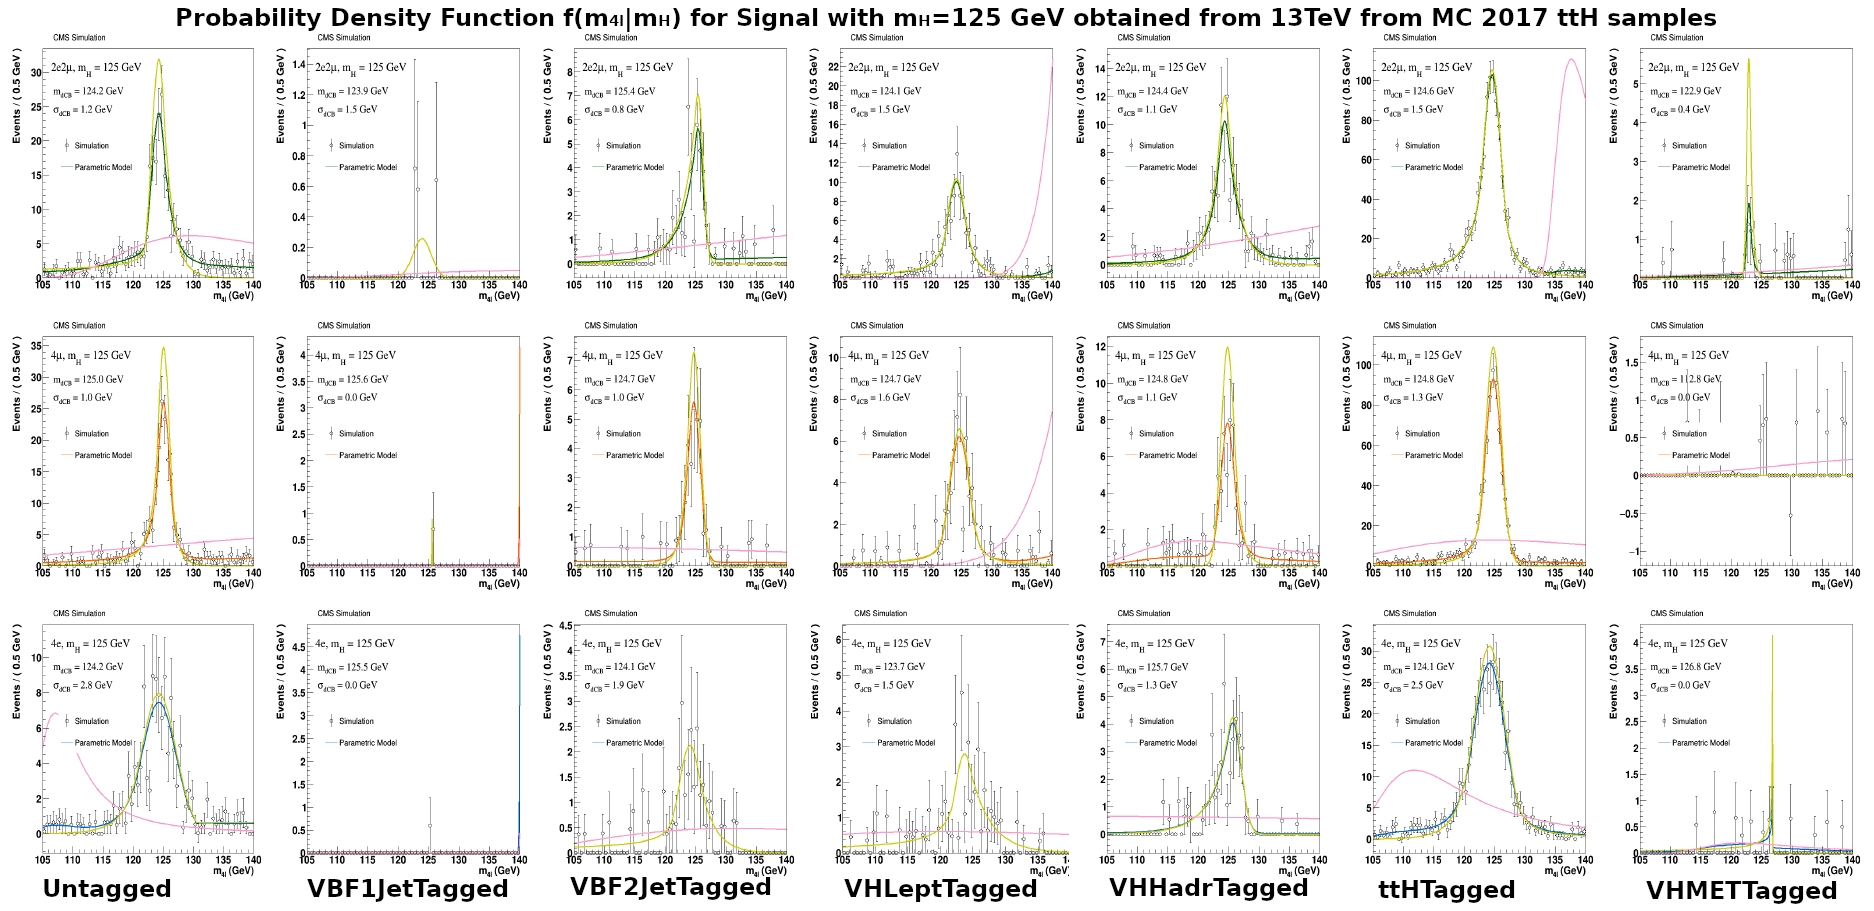
\includegraphics[scale=1]{images/2017.jpg}
    \caption{Sum of probability density functions $f(m_{4l} |m_H)$ for $m_H$ =125 GeV fitted for 13TeV ttH 2017 MC samples.}
    \label{fig:2017}
\end{figure}
\begin{figure}
    \centering
    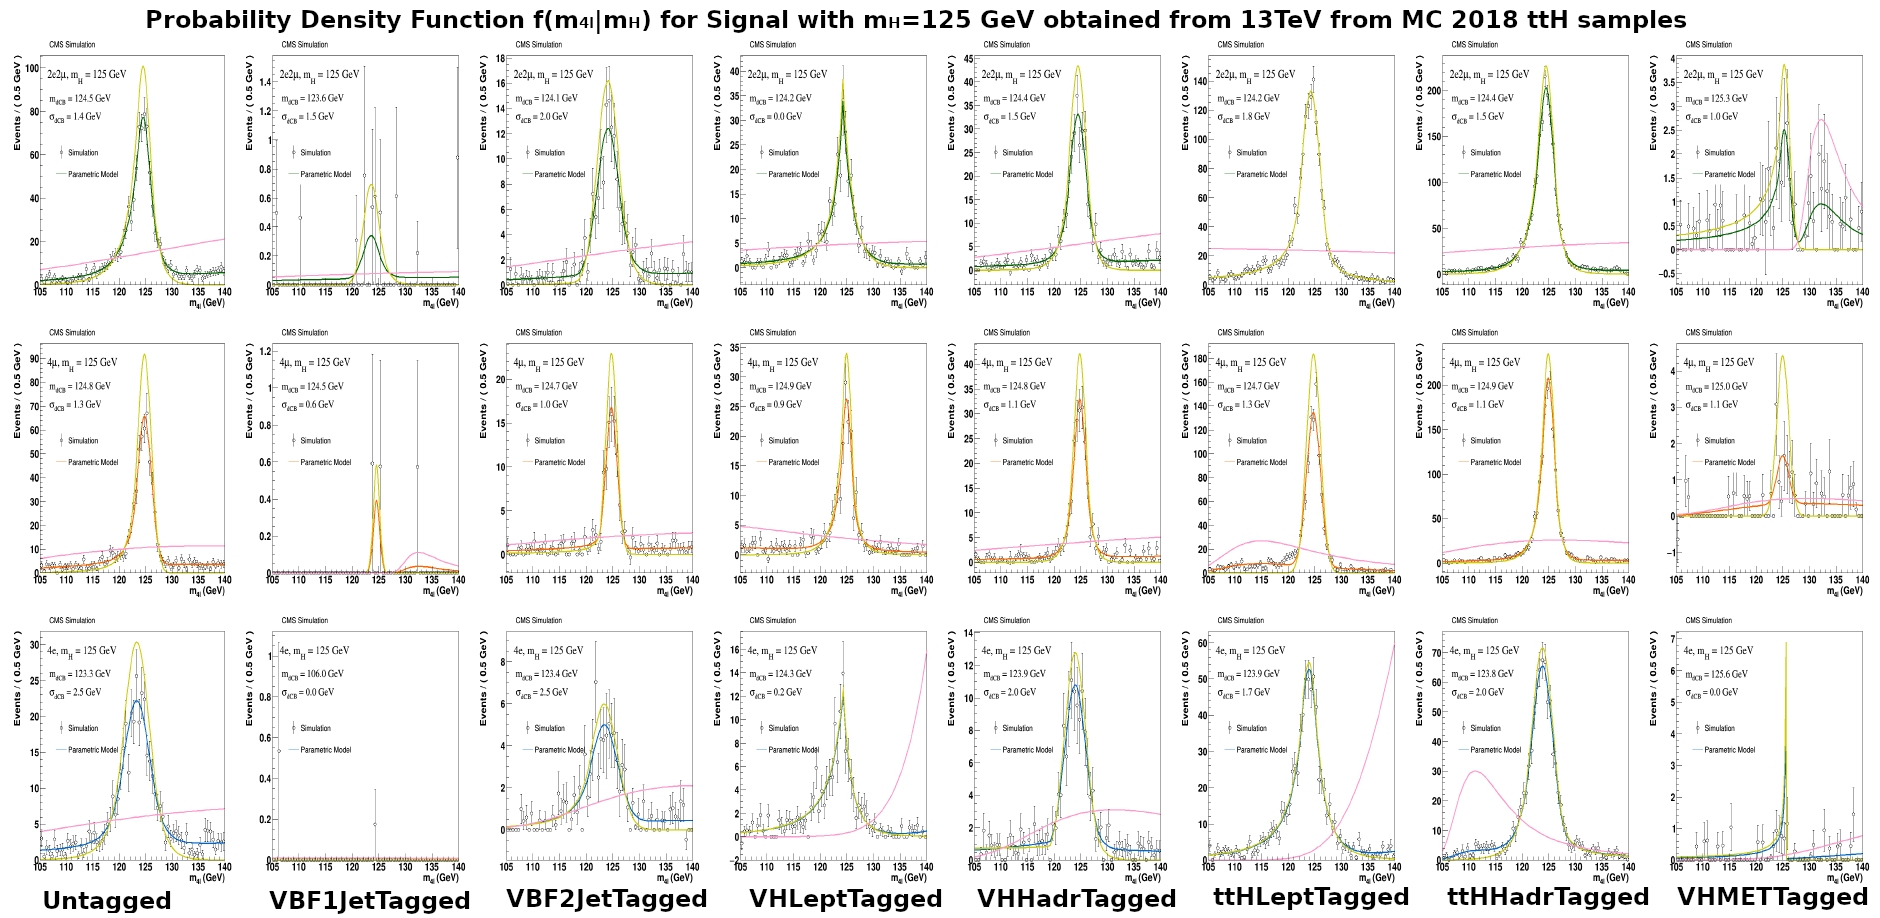
\includegraphics[scale=1]{images/2018.jpg}
    \caption{Sum of probability density functions $f(m_{4l} |m_H)$ for $m_H$ =125 GeV fitted for 13TeV ttH 2018 MC samples.}
    \label{fig:2018}
\end{figure}

\subsection{Signal Yield Parameterization}
The normalization of Higgs Boson signal in $dCB$, described in Eq.\ref{eqn:dcb}, is taken from simulation directly in the peak region. The parameterization of normalization constant N (for a given $m_H$) translates to estimated signal yields. Using simulated samples in $ 105 < m_{4l} < 140$ GeV signal window, for final states, all production modes and all event categories, a polynomial of second order is carried out for $m_H$ points (120, 124, 125, 126 and 130 GeV).\\
\begin{figure}[h]
     \centering
     \begin{subfigure}[b]{0.3\textwidth}
         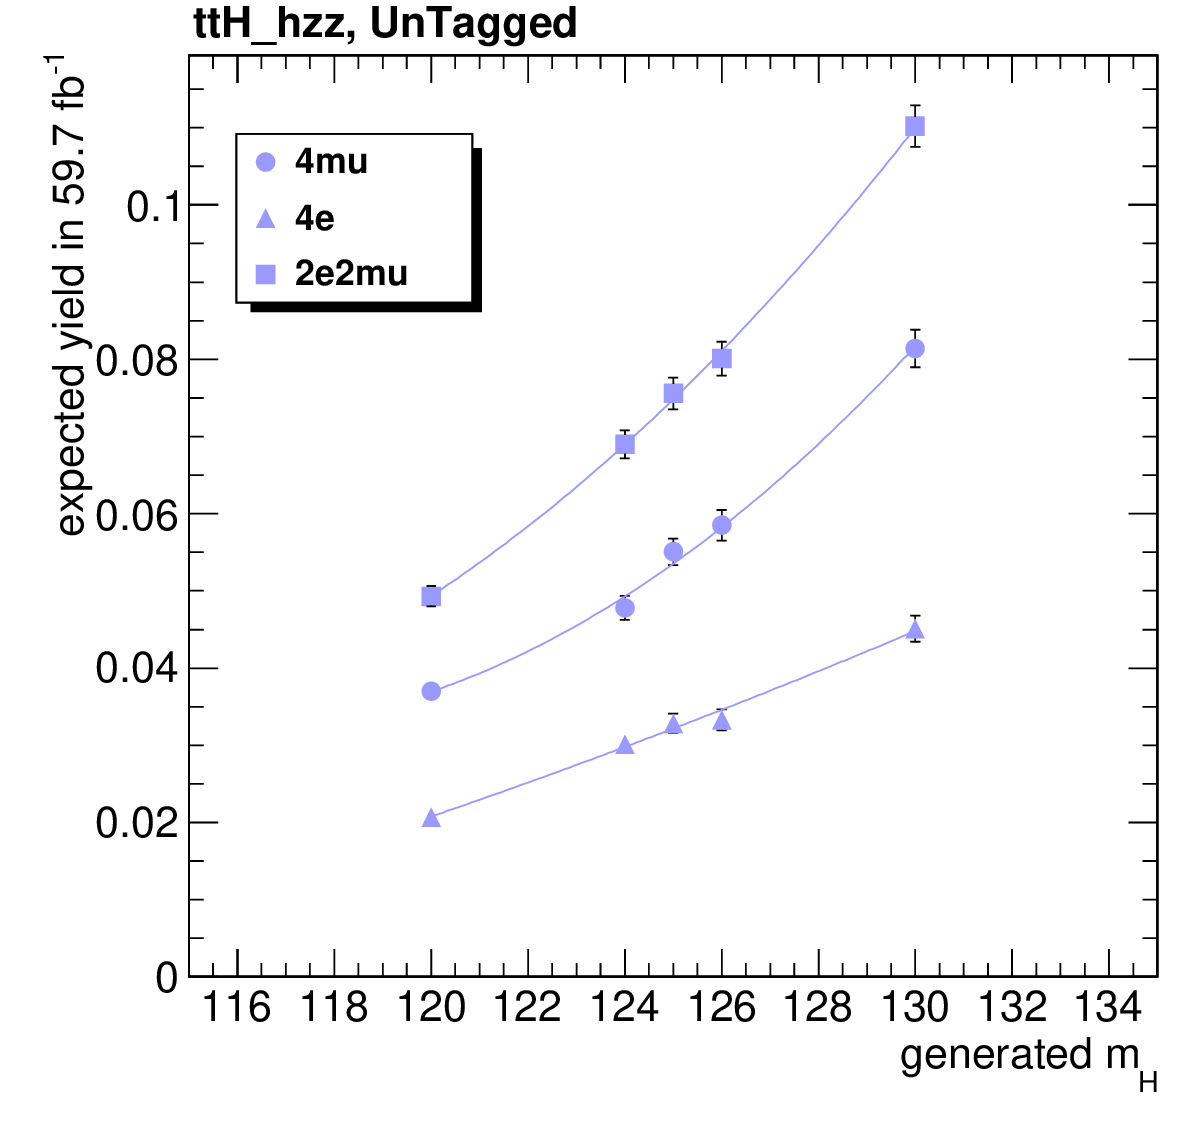
\includegraphics[width=\textwidth]{images/cFits_ttH_hzz_UnTagged_.png}
         \caption{UnTagged Category}
     \end{subfigure}
      \hfill
     \begin{subfigure}[b]{0.3\textwidth}
         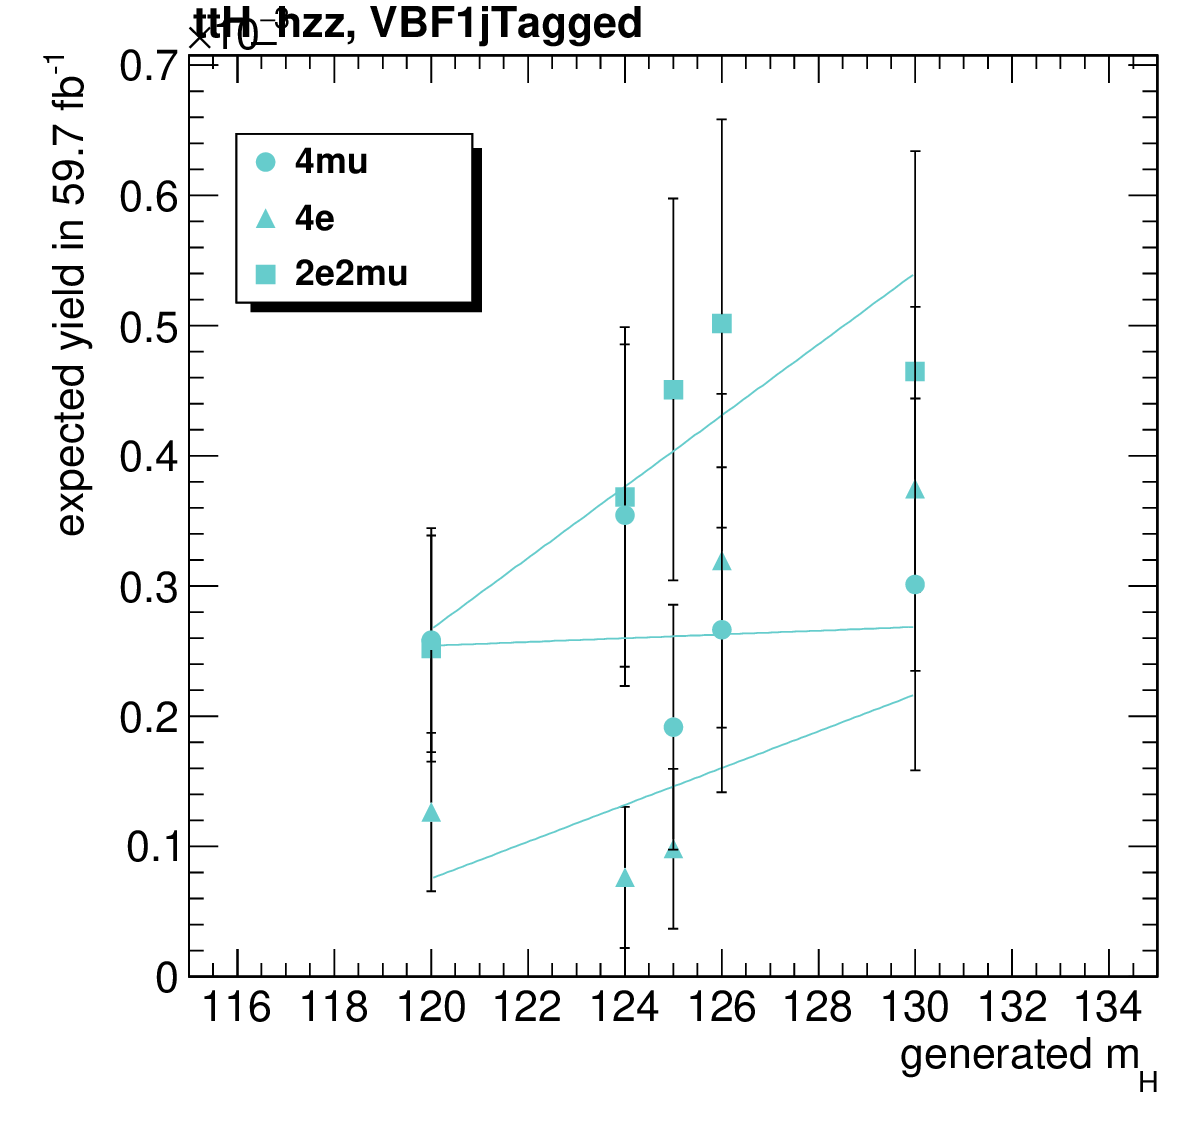
\includegraphics[width=\textwidth]{images/cFits_ttH_hzz_VBF1jTagged_.png}
         \caption{VBF1jTagged Category}
     \end{subfigure}
      \hfill
     \begin{subfigure}[b]{0.3\textwidth}
         
         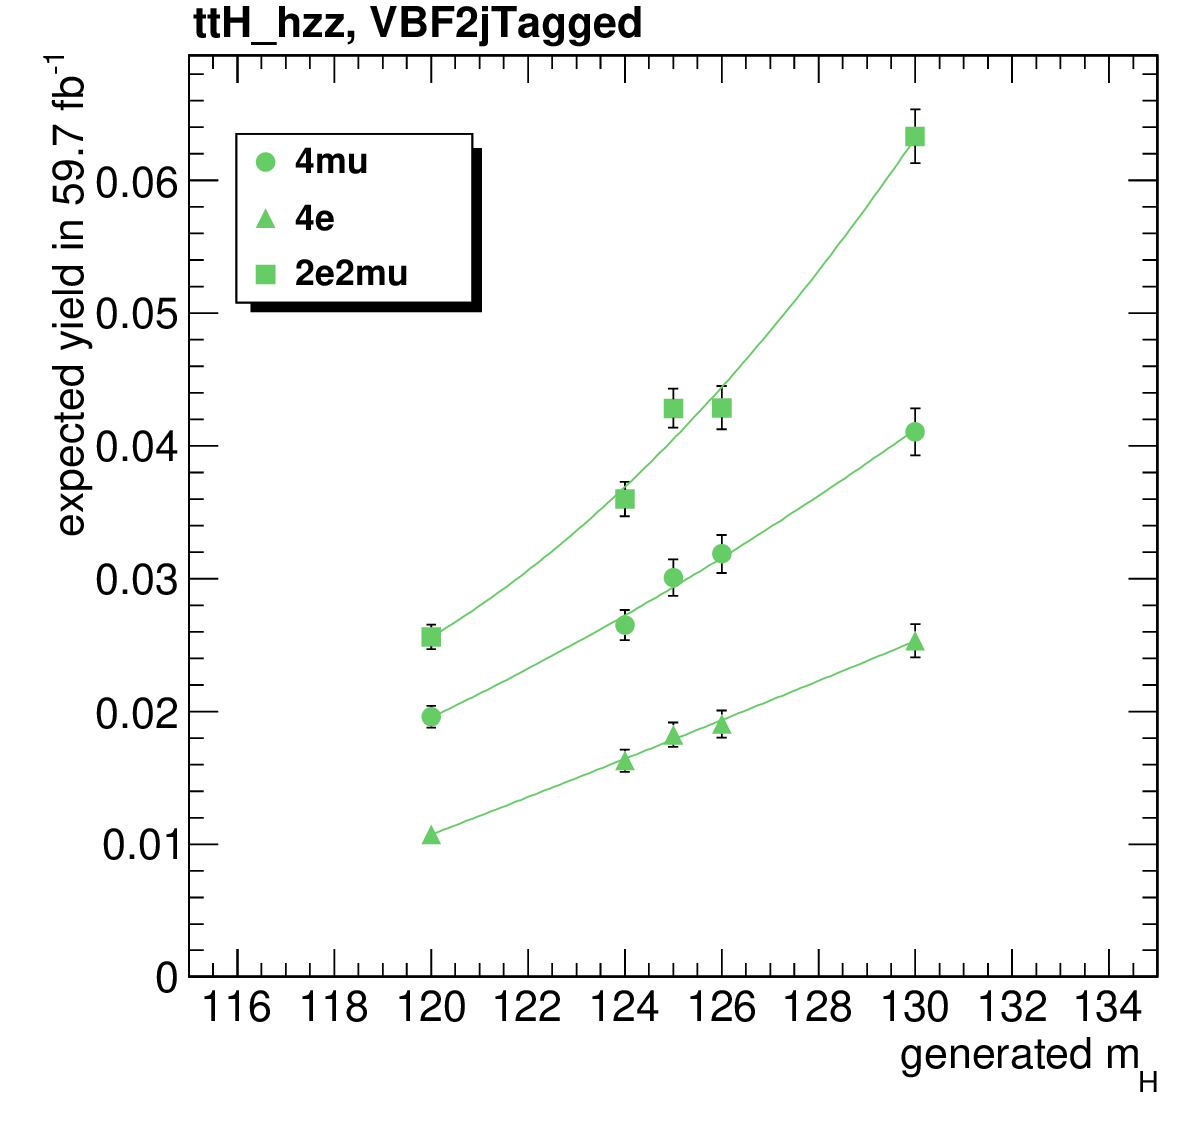
\includegraphics[width=\textwidth]{images/cFits_ttH_hzz_VBF2jTagged_.png}
         \caption{VBF2jTagged Category}
         \end{subfigure}
          \hfill
         \begin{subfigure}[b]{0.3\textwidth}
         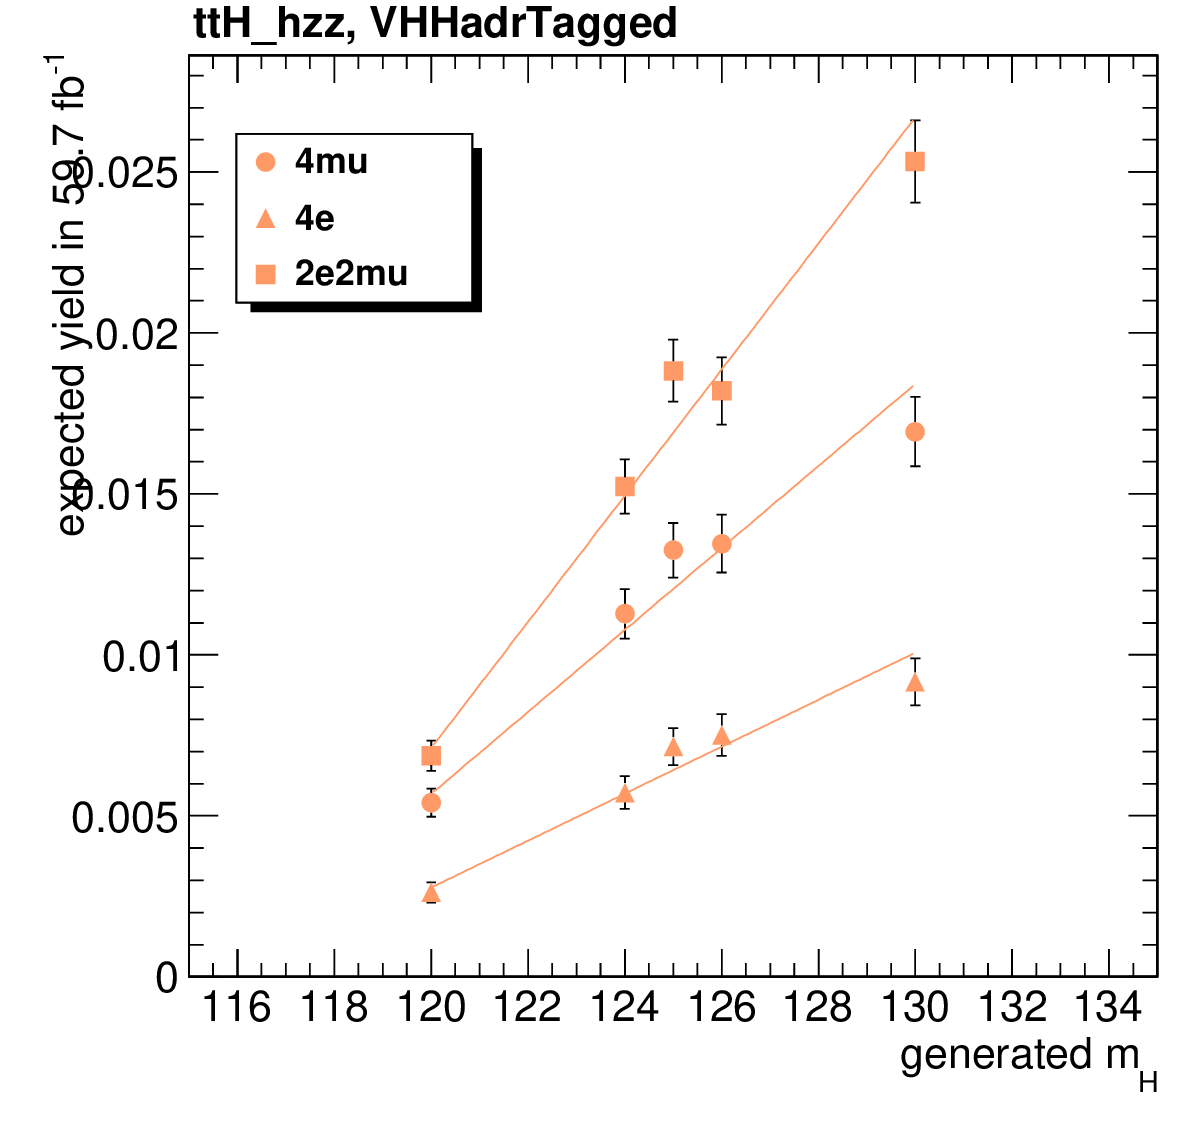
\includegraphics[width=\textwidth]{images/cFits_ttH_hzz_VHHadrTagged_.png}
         \caption{VHHadrTagged Category}
     \end{subfigure}
     \hfill
     \begin{subfigure}[b]{0.3\textwidth}
         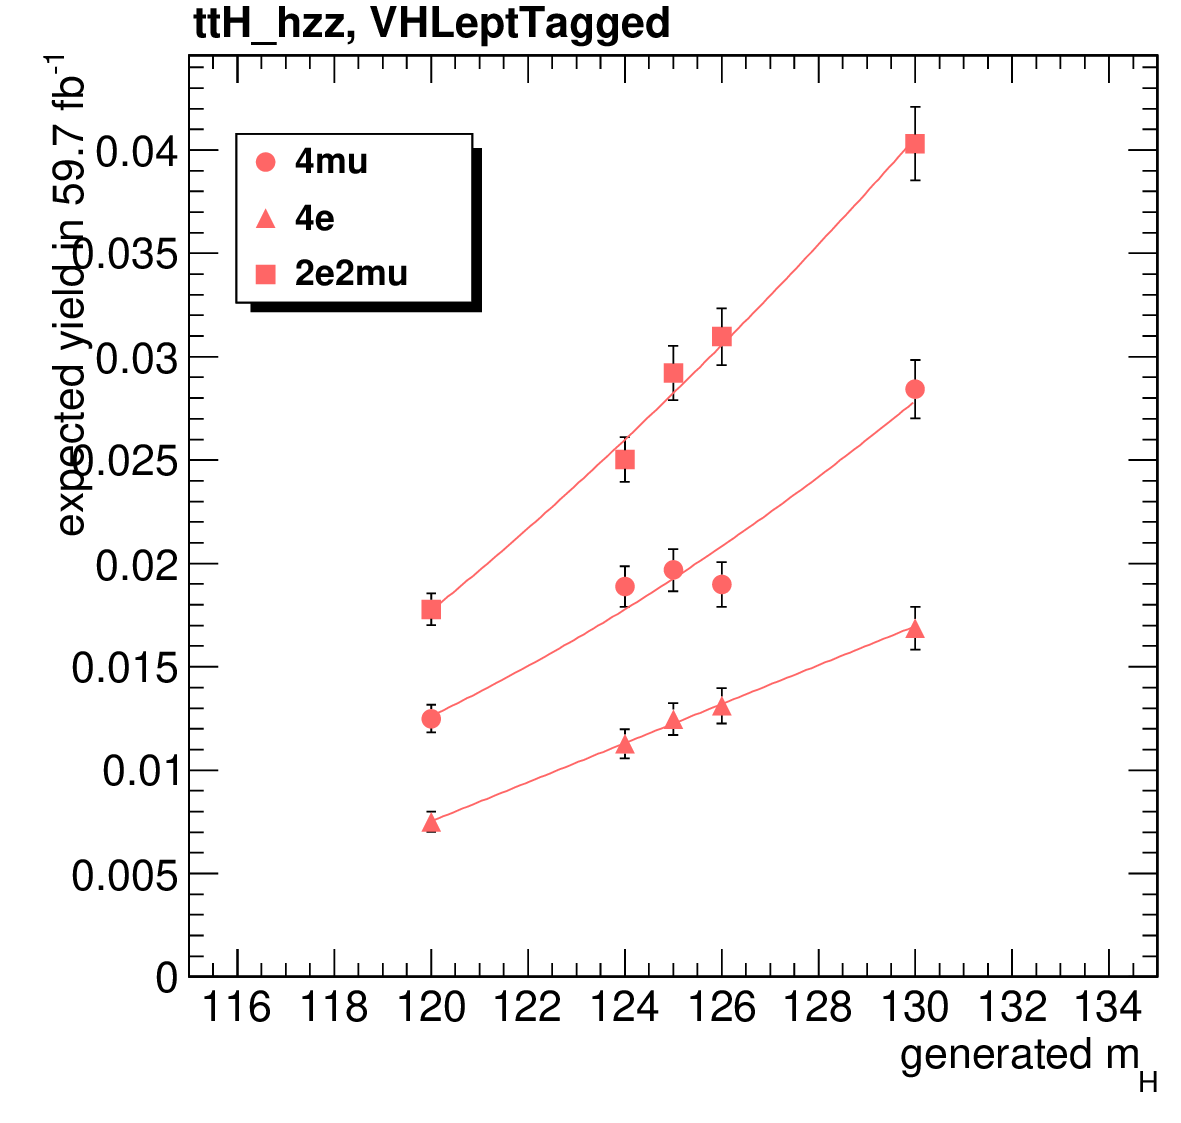
\includegraphics[width=\textwidth]{images/cFits_ttH_hzz_VHLeptTagged_.png}
         \caption{VHLeptTagged Category}
     \end{subfigure}
      \hfill
     \begin{subfigure}[b]{0.3\textwidth}
        
         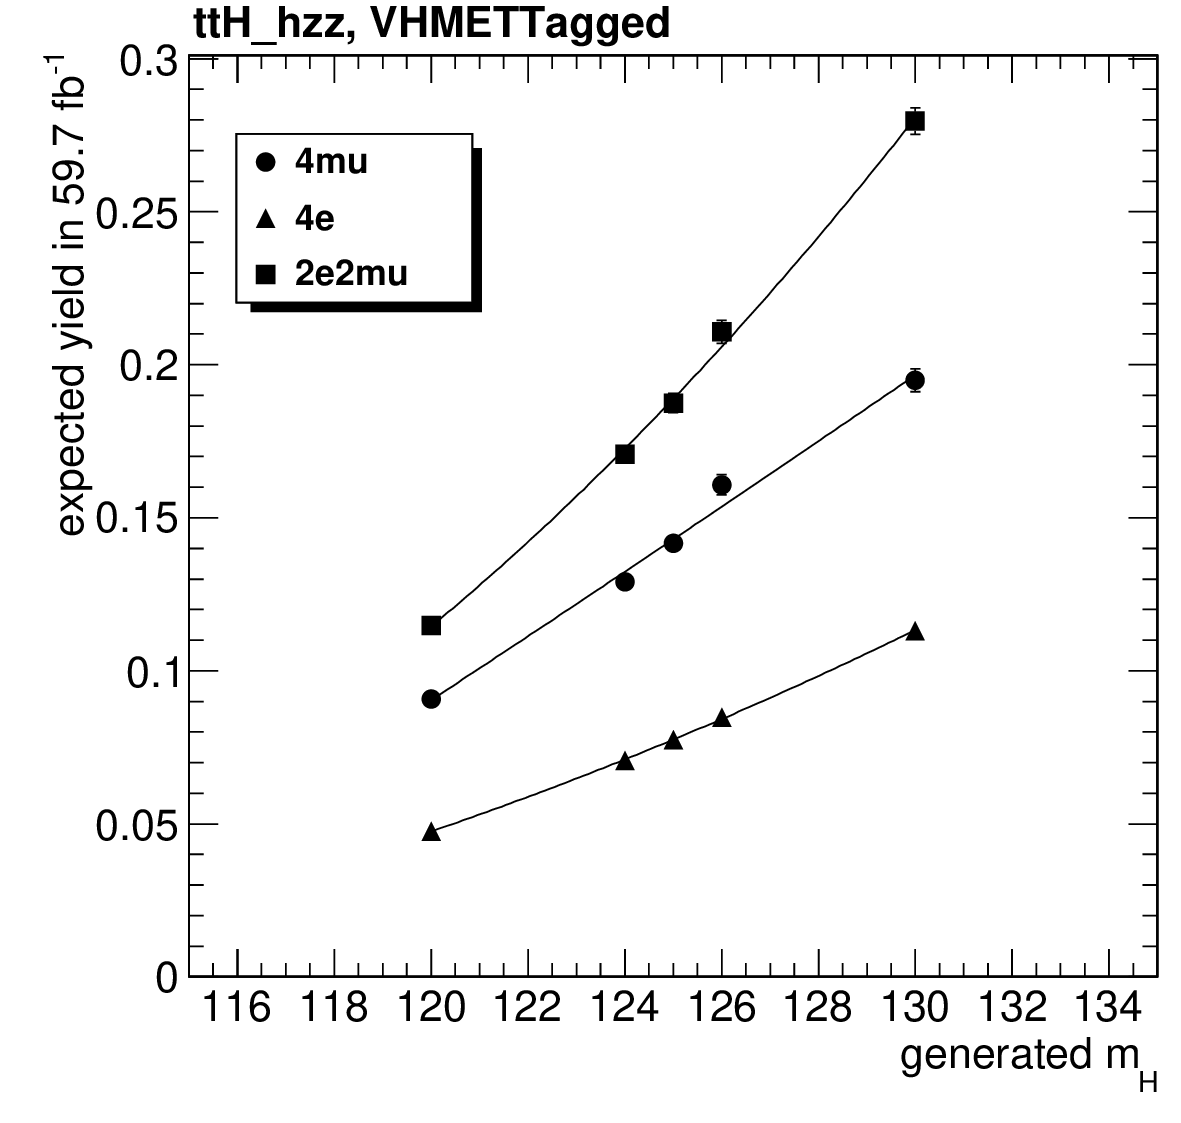
\includegraphics[width=\textwidth]{images/cFits_ttH_hzz_VHMETTagged_.png}
         \caption{VHMETTagged Category}
     \end{subfigure}
       \hfill
        \begin{subfigure}[b]{0.3\textwidth}
         
         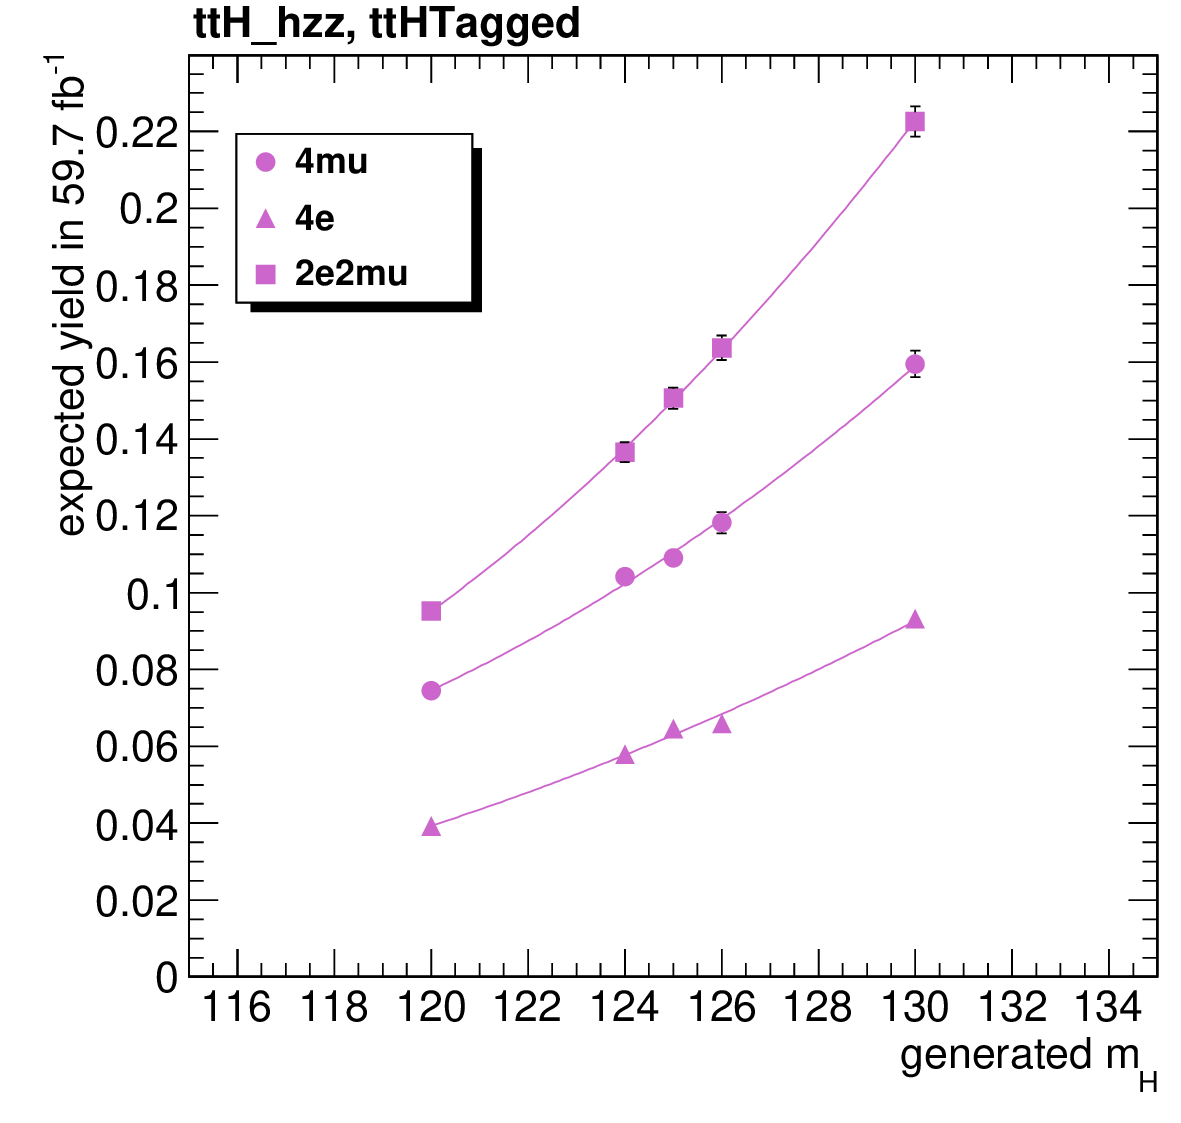
\includegraphics[width=\textwidth]{images/cFits_ttH_hzz_ttHTagged_.png}
         \caption{ttHTagged Category}
         \label{fig:five over x}
     \end{subfigure}
        \caption{Expected signal yields fits after full event
selection in a [105, 140] GeV $m_{4l}$ window, for the ttH production mode in the 2018 seven event category for an integrated luminosity of 59.7 fb$^{-1}$.}
        \label{fig:yield}
\end{figure}
A numerical analysis; spline interpolation, is used, which is a type of interpolation where interpolant is a form of piece-wise polynomial called a spline. It is given preference over polynomial interpolation as it can give similar results, with lesser degree polynomials.
Fits of the expected signal yields depended on $m_H$ for 59.7 $fb^{-1}$ in the $105 < m_{4l} < 140$ GeV range after fully selecting events, are parameterized in the range $118 < m_{4l} < 134$ GeV for 2018 MC data in Fig:\ref{fig:yield}.

\subsection{Signal Background Parameterization}
There are two kinds of background, the ``\textbf{reducible}'' backgrounds where particles fake the particles we are looking for (for example, a high energy electron can look just like a high energy photon) and the ``\textbf{irreducible}'' backgrounds where particles are the same kind as the ones we are looking for. 
\begin{itemize}
    \item \textbf{Irreducible} backgrounds which come from the production of $ZZ$ via quark anti-quark annihilation or gluon fusion, are estimated using simulation.
    \item  \textbf{Reducible} background is estimated using two independent methods having dedicated control regions in data.
\end{itemize}
During the study of $H \rightarrow Z Z^* \rightarrow 4l$, major irreducible backgrounds were from fusion of two gluons $gg \rightarrow ZZ$ and annihilation of quark anti-quark pair $q \bar{q} \rightarrow ZZ$ where $Z$ bosons decay into a lepton pair. In both cases, no intermediary Higgs boson is detected, Z boson pair is directly produced. The kinematics discriminant and expected yield are obtained from simulations by estimation of irreducible backgrounds.\\
\begin{figure}[h]
    \centering
    \begin{subfigure}[b]{0.8\textwidth}
     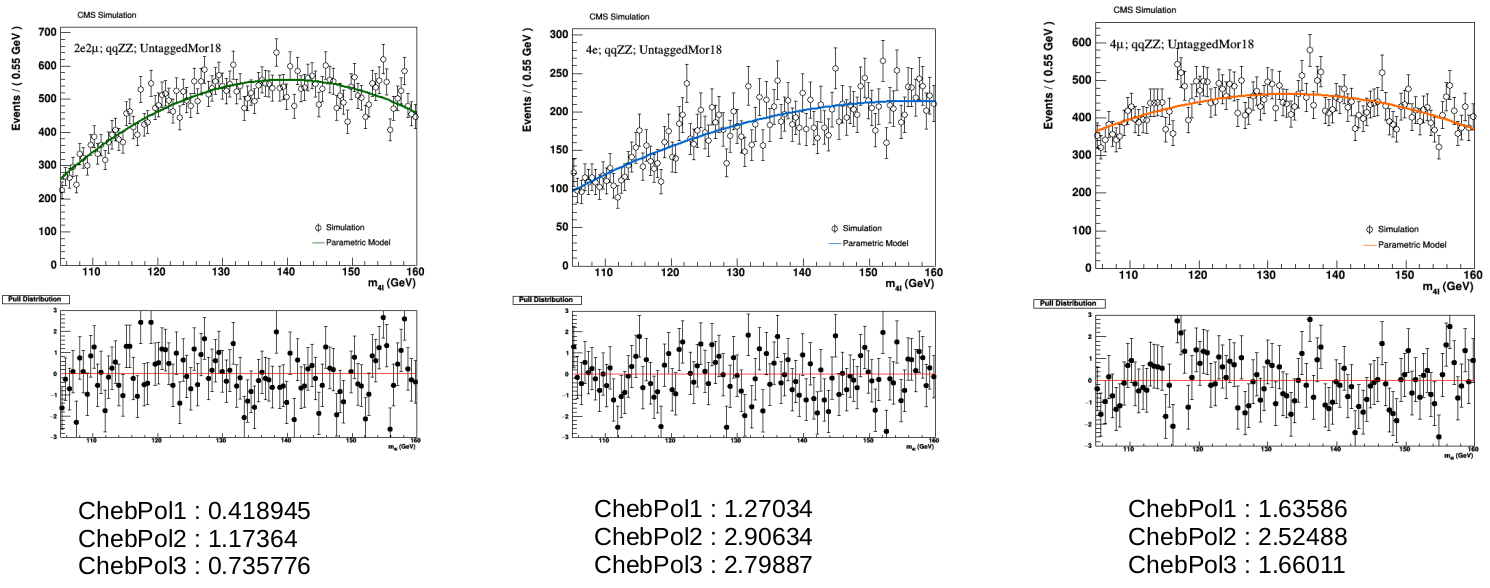
\includegraphics[width=\textwidth]{images/be.png}
     \caption{fusion of gluons $gg \rightarrow ZZ$}
     \label{fig:gg}
    \end{subfigure}
    \vfill
    \begin{subfigure}[b]{0.8\textwidth}
    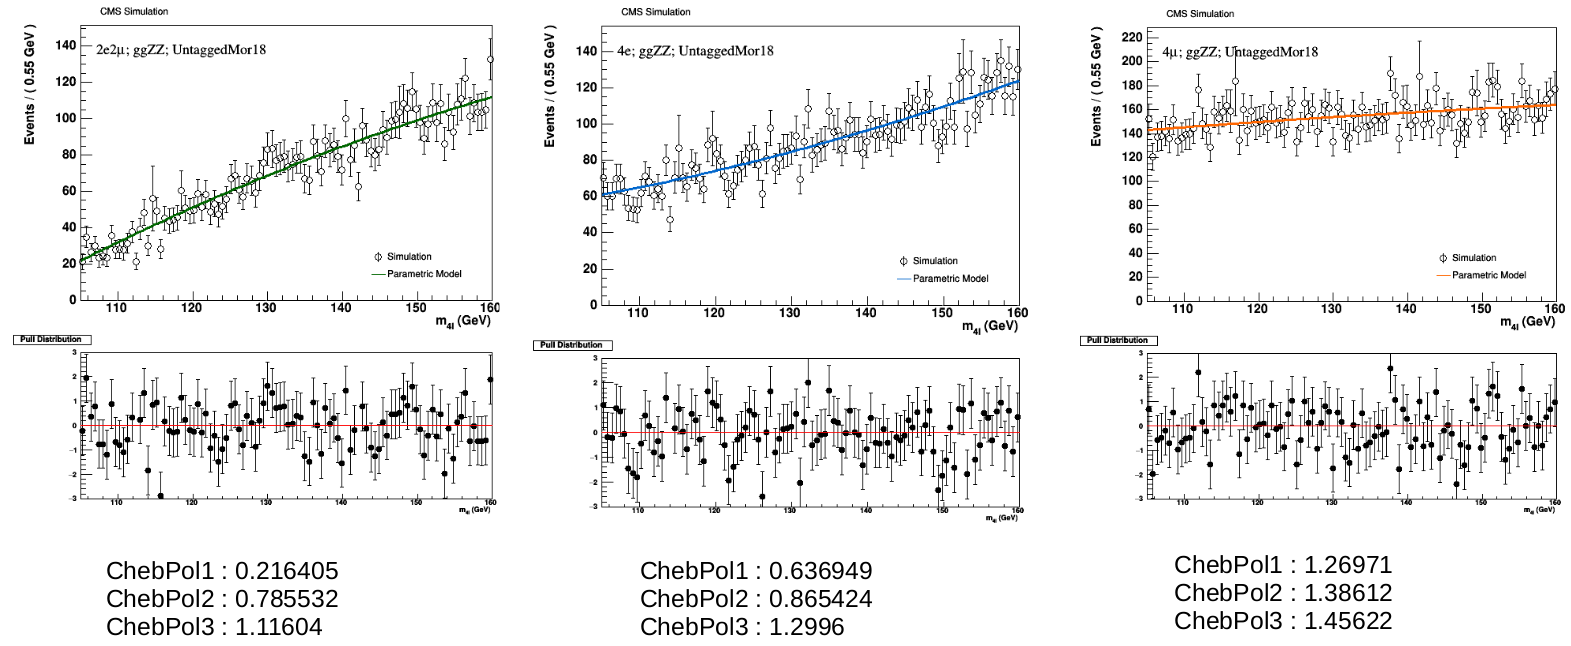
\includegraphics[width=\textwidth]{images/be1.png}
    \caption{annihilation quark anti-quark $q \bar{q} \rightarrow ZZ$ }
     \label{fig:qq}
    \end{subfigure}
     \caption{Irreducible background fitting using Chebyshev's polynomials.}
    \label{fig:be}
\end{figure}
We have used third order Chebyshev's polynomials ``ChebPol'' explained in detail in section \ref{section:cp}. It is a multivariate interpolation, which contains methods for creating multivariate/multidimensional interpolations of functions on a hypercube. Examples for gluon fusion $gg \rightarrow ZZ$ in Fig.\ref{fig:gg} and quark antiquark annihilation $q \bar{q} \rightarrow ZZ$ in Fig.\ref{fig:qq} for 2018 data analysis in untagged category for 3 final states 4$\mu$, 4e and 2e2$\mu$ are illustrated as well as first three Chebyshev's polynomials with their pull distribution.\\
All categories for 2016, 2017 and 2018 data irreducible background is given in appendix \ref{appendix:be}.
\clearpage
\subsection{Results of Event Selection}
The events and their number observed in data with their yields for 35.9 fb$^{-1}$, 41.5 fb$^{-1}$ and 59.7 fb$^{ -1}$ of data collected in 2016,2017 and 2018 for Higgs signal and backgrounds after complete event reconstruction are reported in Table: \ref{tab:es6}, \ref{tab:es7} and \ref{tab:es8} for the full range of $m_{4l}$.
\begin{table}
    \centering
   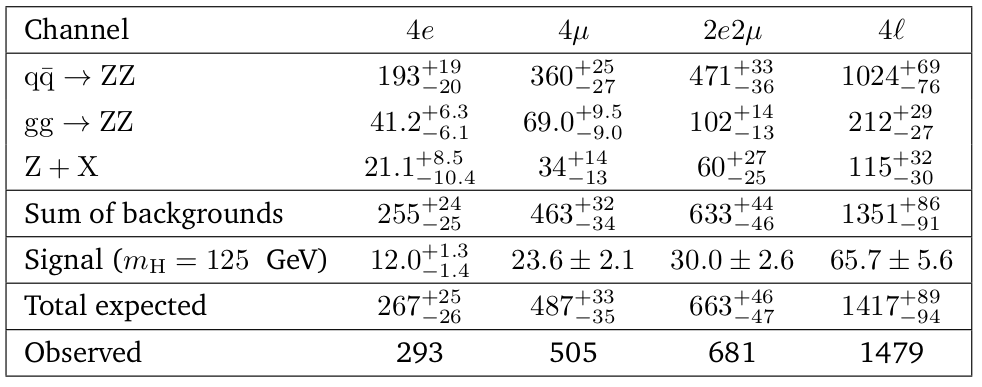
\includegraphics[scale=0.4]{images/es6.png}
    \caption{Event's number for an integrated luminosity of 35.9 fb$^{-1}$.}
    \label{tab:es6}
\end{table}
\begin{table}
    \centering
   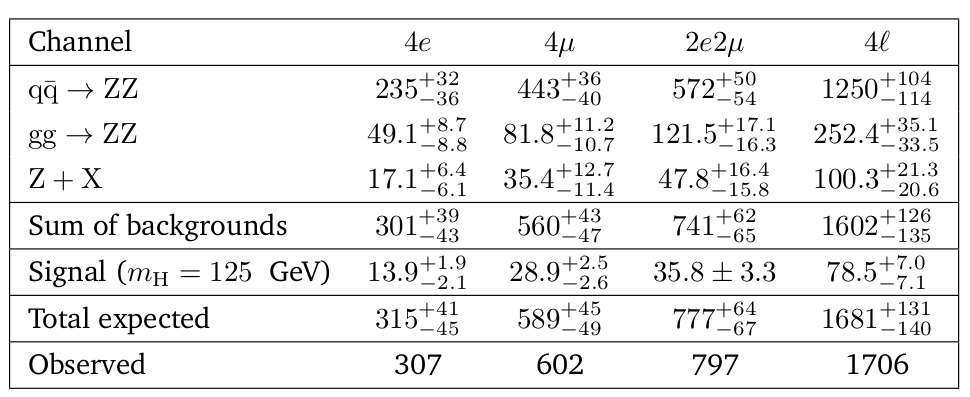
\includegraphics[scale=0.4]{images/es7.png}
    \caption{Event's number for an integrated luminosity of 41.5 fb$^{-1}$.}
    \label{tab:es7}
\end{table}
The estimated background and signal events numbers as well as observed candidates numbers are calculated after full event reconstruction, in every final state for mass range $m_{4l} >70$ GeV. Signal and ZZ background are calculated from MC simulation, while Z +X is calculated directly from data.\\
The error bars at every value are the so-called Garwood confidence intervals at 68$\%$ confidence level (CL) \cite{<fg>}. The expected distribution and observed distribution are in agreement within the statistical uncertainties over the whole spectrum.
\begin{table}
    \centering
   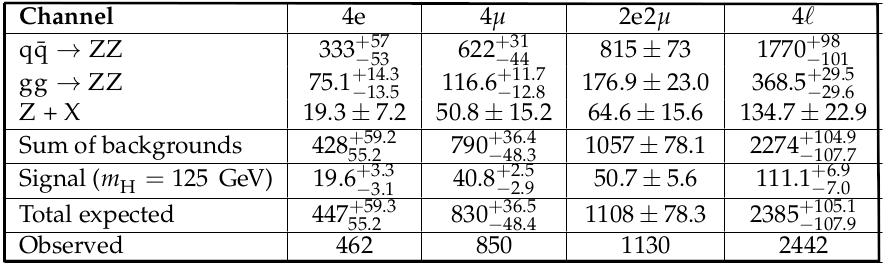
\includegraphics[scale=0.4]{images/es8.png}
    \caption{Event's number for an integrated luminosity of 59.7 fb$^{-1}$.}
    \label{tab:es8}
\end{table}

\section{Signal Strength Modifier Measurement}
The signal strength modifier $\mu$ is defined as the ratio of measured Higgs boson rate to the predicted theoretical Higgs boson rate in the SM, which categorizes Higgs boson yields. For a distinct production and decay mode $i \rightarrow H \rightarrow f$ the signal strength of production, $\mu_i$ is given by,
\begin{equation}
    \mu_i = \frac{\sigma_i}{(\sigma_i)_{SM}}, \hspace{5mm} and  \hspace{5mm}  \mu^f = \frac{B^f}{(B^f)_{SM}}
\end{equation}
Here, $\sigma_i$ ($i$=ggH,VBF,WH,ZH,t$\bar{t}$H) are production cross sections for $i \rightarrow H$ and $B^f$ ($f=ZZ$) as we consider only the golden channel, is the decay branching ratio $H \rightarrow f$. The subscript SM represents the corresponding predicted SM values, which are $\mu_i$=1 and $\mu^f$=1. The product of $\mu_i$ and $\mu^f$ can be experimentally measured, leading to signal strength $\mu^f_i$ for combined production and decay;
\begin{equation}
    \mu^f_i = \frac{\sigma_i . B^f }{(\sigma_i)_{SM} . (B^f)_{SM}} = \mu_i . \mu^f
\end{equation}
To exploit all the properties of the resonance under study or search, a multi-dimensional fit is implemented. For every category described in
section \ref{section:ec}, two variables are taken in consideration for the maximum likelihood fit, namely:
\begin{enumerate}
    \item The four-lepton mass $m_{4l}$,
    \item The kinematic discriminant $D^{kin}_{bkg}$.
\end{enumerate}
To account for the strong correlation of the kinematic discriminant with
the mass, a 2D histogram template of $D^{kin}_{bkg}$ vs. $m_{4l}$ is implemented. Due to the small number of expected events in the mass peak, the unbinned data (fitted data except goodness of fit) is used for mass dimension and the resolution model is used as described in section \ref{section:smm}. The total PDF is defined as:
\begin{equation}
    \mathcal{L}_{2D} (m_{4l}) = \mathcal{L} (m_{4l}) \mathcal{L} (D^{kin}_{bkg} | m_{4l})
    \label{eqn:mdf}
\end{equation}
where the first factor corresponds to the 1D mass PDF and the second factor
to the 2D template of mass vs. kinematic discriminant. The conditional term
in the second factor is implemented in the template by normalizing all $D^{kin}_{bkg}$ columns corresponding to the same mass value each. Therefore, the 2D template does not include any information on the mass, but given the mass, it provides information on the kinematic discriminant.\\
In this section, we describe the method used for estimation of the signal strength, i.e. its total cross section normalized to the one expected for a SM Higgs. A multi-dimensional fit is implemented as explained by the Eq.\ref{eqn:mdf}.
These results are compatible with SM expectations under the uncertainties, which in our current events are majorly statistical. The results are compared to the expected signal-strength modifiers in Table.\ref{tab:tab2018}.
\begin{table}[]
    \centering
    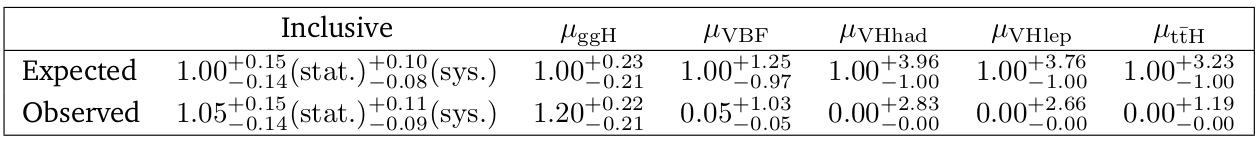
\includegraphics[width=\textwidth]{images/tab2016.png}
    \caption{Expected and observed signal strength modifier at 35.9 fb$^{-1}$.}
    \label{tab:tab2016}
\end{table}
\begin{table}[]
    \centering
    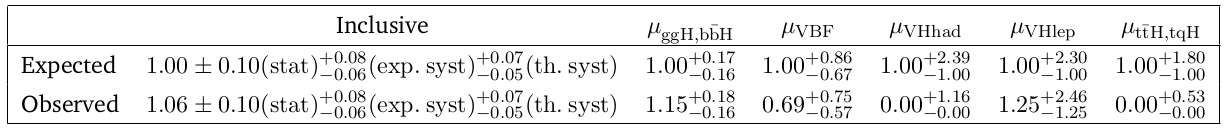
\includegraphics[width=\textwidth]{images/tabcomb.png}
    \caption{Expected and observed signal strength modifier at 77.4 fb$^{-1}$.}
    \label{tab:comb}
\end{table}
\begin{table}
\centering
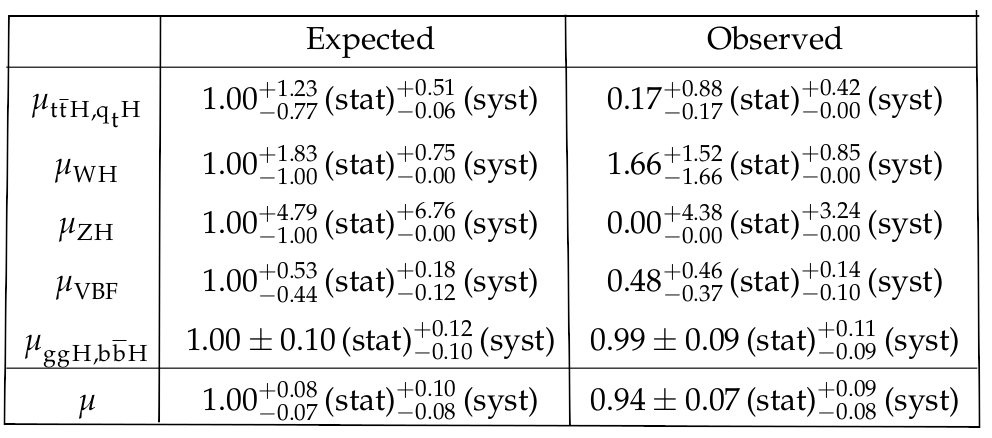
\includegraphics[scale=0.3]{images/tab2018.png}
\caption{Expected and observed signal strength modifier at 137.1 $^{-1}$. \cite{<colab2>}}
\label{tab:tab2018}
\end{table}
Two signal-strength modifiers for the five main Higgs production modes are calculated as scale factors for vector boson and fermionic contribution to the expected SM cross section. A two-dimensional fit is executed by the CMS collabortion \cite{<colab1>,<colab2>}, fixing the mass to $m_H = 125.38 GeV$ and profiling the likelihood for all nuisance parameters, leading to the results illustrated in the top row of Fig.\ref{fig:mss}, where $\mu_{WH}$ and $\mu_{ZH}$ are split into leptonically decaying bosons $\mu_{WHlep}$ /$\mu_{ZHlep}$ and hadronically decaying bosons
$\mu_{WHhadr}$ /$\mu_{ZHhadr}$. Also the $\mu_{ttH}$ splits into leptonically decaying fermions $\mu_{ttHlept}$ and hadronically decaying fermions $\mu_{ttHhadr}$. The 68$\%$ and 95$\%$ CL contours in the ($\mu_{ggH,ttH,bbH,qtH}, \mu_{VBF,VH}$) plane are shown in bottom row of Fig.\ref{fig:mss}.
\begin{figure}[h]
     \centering
     \begin{subfigure}[b]{0.3\textwidth}
         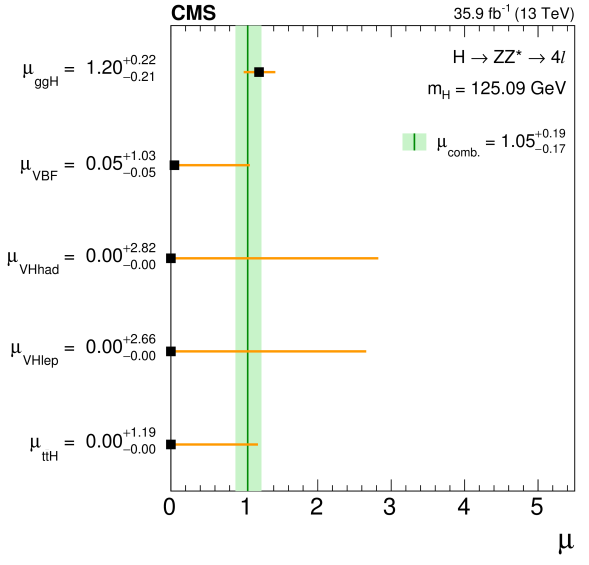
\includegraphics[width=\textwidth]{images/ssm2016.png}
         \caption{2016 observed values}
     \end{subfigure}
      \hfill
     \begin{subfigure}[b]{0.3\textwidth}
         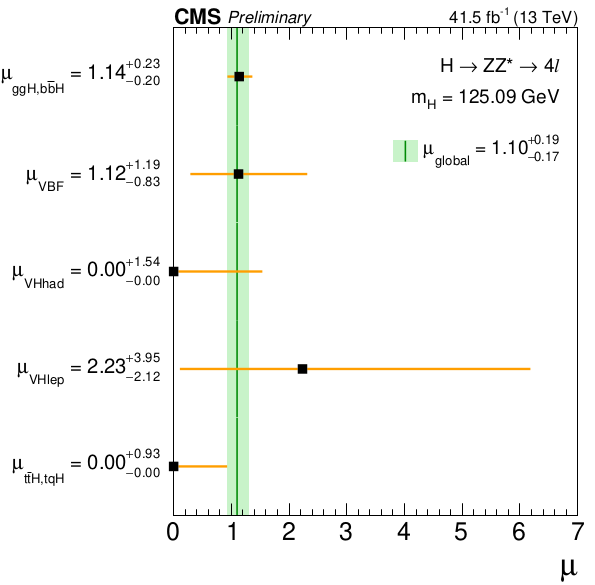
\includegraphics[width=\textwidth]{images/2017ssm.png}
         \caption{2017 observed values}
     \end{subfigure}
      \hfill
     \begin{subfigure}[b]{0.3\textwidth}
         
         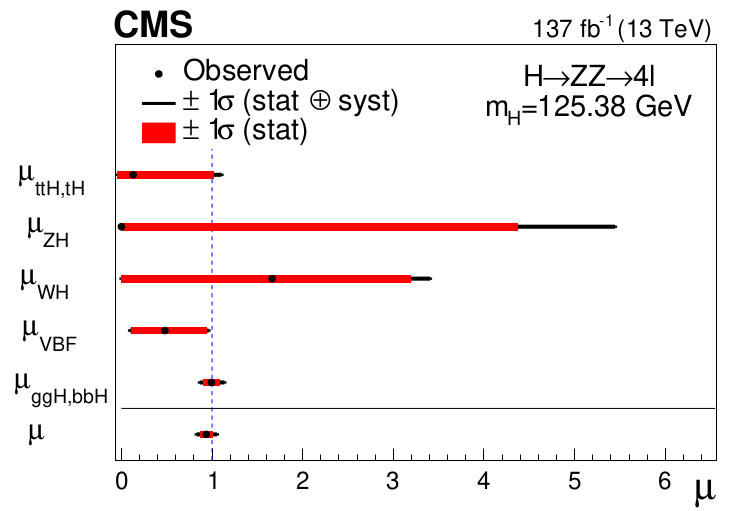
\includegraphics[width=\textwidth]{images/ssm2018.png}
         \caption{2018 observed values}
         \end{subfigure}
          \hfill
         \begin{subfigure}[b]{0.3\textwidth}
         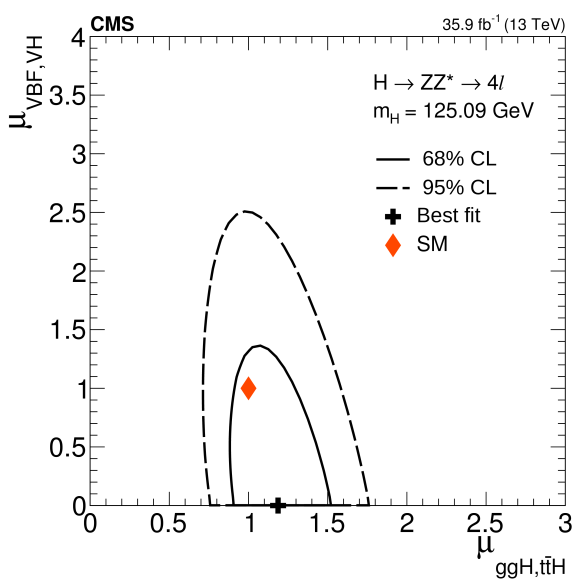
\includegraphics[width=\textwidth]{images/ssm2016b.png}
         \caption{2016 2D likelihood}
     \end{subfigure}
     \hfill
     \begin{subfigure}[b]{0.3\textwidth}
         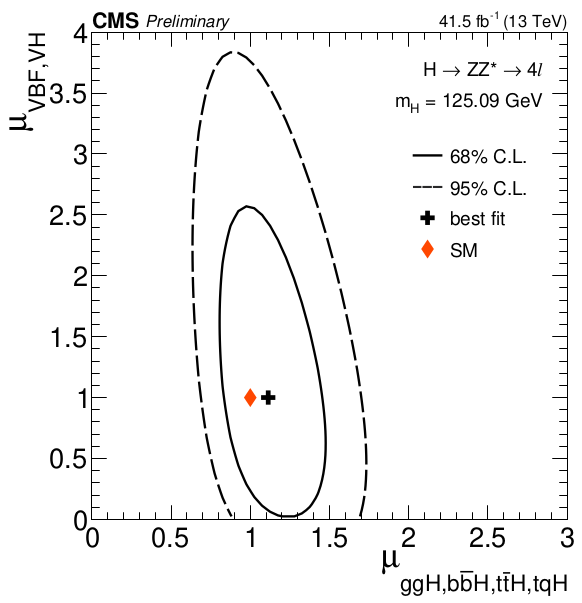
\includegraphics[width=\textwidth]{images/2017ssmb.png}
         \caption{2017 2D likelihood}
     \end{subfigure}
      \hfill
     \begin{subfigure}[b]{0.3\textwidth}
        
         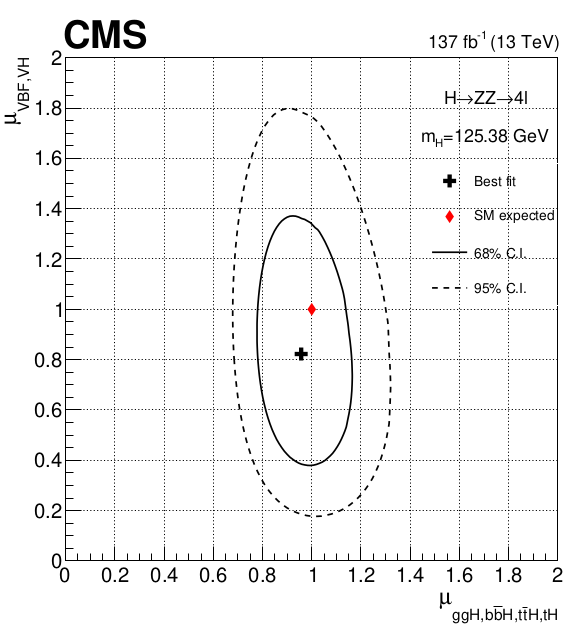
\includegraphics[width=\textwidth]{images/ssm2018b.png}
         \caption{2018 2D likelihood}
     \end{subfigure}
        \caption{Observed values, in each event category, of the signal strength $\mu = \sigma / \sigma_{SM}$, where the vertical line shows combined $\mu$. $\pm 1\sigma$ uncertainties can be seen as filled band along horizontal bars (top row). A likelihood in 2D space for the $\mu_{fermionic}$ and $\mu_{bosonic}$. The dashed and solid contours illustrate 68$\%$ and 95$\%$ CL regions, respectively. The diamond shows the expected values for the SM Higgs boson where as the cross points to the best-fit values (bottom row). \cite{<colab1>,<colab2>}}
        \label{fig:mss}
\end{figure}